
\documentclass[svgnames]{beamer}

\mode<presentation> {
\usetheme{Warsaw}
}

\usepackage{graphicx}
\usepackage{booktabs}
\usepackage{listings}
\usepackage{color}
%\usepackage[lofdepth,lotdepth]{subfig}
\usepackage{subfig}
\usepackage{fontawesome}
\usepackage{hyperref}

\definecolor{codegreen}{rgb}{0,0.6,0}
\definecolor{codegray}{rgb}{0.5,0.5,0.5}
\definecolor{codepurple}{rgb}{0.58,0,0.82}
\definecolor{backcolour}{rgb}{0.95,0.95,0.92}

\beamertemplatenavigationsymbolsempty


\lstdefinestyle{mystyle}{
    backgroundcolor=\color{backcolour},   
    commentstyle=\color{codegreen},
    keywordstyle=\color{magenta},
    numberstyle=\tiny\color{codegray},
    stringstyle=\color{codepurple},
    %basicstyle=\footnotesize,
    basicstyle=\scriptsize\ttfamily,
    breakatwhitespace=false,         
    breaklines=true,                 
    captionpos=b,                    
    keepspaces=true,                 
    numbers=left,                    
    numbersep=5pt,                  
    showspaces=false,                
    showstringspaces=false,
    showtabs=false,                  
    tabsize=2,
    language=bash
}



\lstset{style=mystyle}

% \newcommand{\SubItem}[1]{
%     {\setlength\itemindent{15pt} \item[-] #1}
% }

%------------
%	TITLE PAGE
%------------

\title[Version control, Git, GitHub and GitFlow]{Introduction to Git and GitFlow} 
\author{Criscely Luj\'{a}n \\ criscely.lujan@ird.fr \\ \and
Nicolas Barrier \\
nicolas.barrier@ird.fr}
\institute[Universit\'{e} Paris-Sud, UMR MARBEC]  
{Universit\'{e} Paris-Sud, UMR MARBEC \\ 
\medskip
\textit{criscely.lujan@ird.fr}
}
\author[Criscely Luj\'{a}n \& Nicolas Barrier]{Criscely Luj\'{a}n\inst{1,2} \\ \vspace{-0.5em} \tiny \emph{\href{mailto:criscely.lujan@ird.fr}{criscely.lujan@ird.fr}} \normalsize \\ \vspace{1em}
                         \and Nicolas Barrier\inst{2}\\  \tiny \emph{\href{mailto:nicolas.barrier@ird.fr}{nicolas.barrier@ird.fr}}}
\institute[shortinst]{\inst{1} Universit\'{e} Paris-Sud, UMR MARBEC \and \inst{2} IRD, UMR MARBEC}

\date{April 11, 2019}

\hypersetup{
    colorlinks=true,
    linkcolor=white,
    urlcolor=blue,
}

\begin{document}

%------------
\begin{frame}
    \titlepage 
    \begin{center}
        
\includegraphics[height=1.5cm]{img/logo_psud.jpg}
        \hspace{1em}
        
\includegraphics[height=1.5cm]{img/logo_marbec.png}
        \hspace{1em}
        
\includegraphics[height=1.5cm]{img/logo_ird.png}
    \end{center}
\end{frame}

\begin{frame}
    \frametitle{Version control}

    Also known as \textbf{revision control} or \textbf{source control}. \hfill \break

    ... ``\textit{is the management of changes:}

    \begin{itemize}
        \item \textit{documents
        \item computer programs
        \item large web sites
        \item other collections of information ... }''
    \end{itemize}
\end{frame}


\begin{frame}
    \frametitle{Why version control is important?}
    \begin{center}
        
\includegraphics[scale=0.29]{img/phd_comics.png}
    \end{center}
\end{frame}


\begin{frame}
\frametitle{Why version control is important?}

Storing \textbf{version} (properly). 
  \begin{itemize}
    \item [$-$] Saving successive changes (``commit")
    \item [$-$] Versioning (v0.1)
  \end{itemize}


\begin{center}

\includegraphics[scale=0.15]{img/storingVersion.jpg}
\end{center}

\end{frame}


\begin{frame}
\frametitle{Why version control is important?}
\textbf{Restoring} previous versions.

\begin{center}
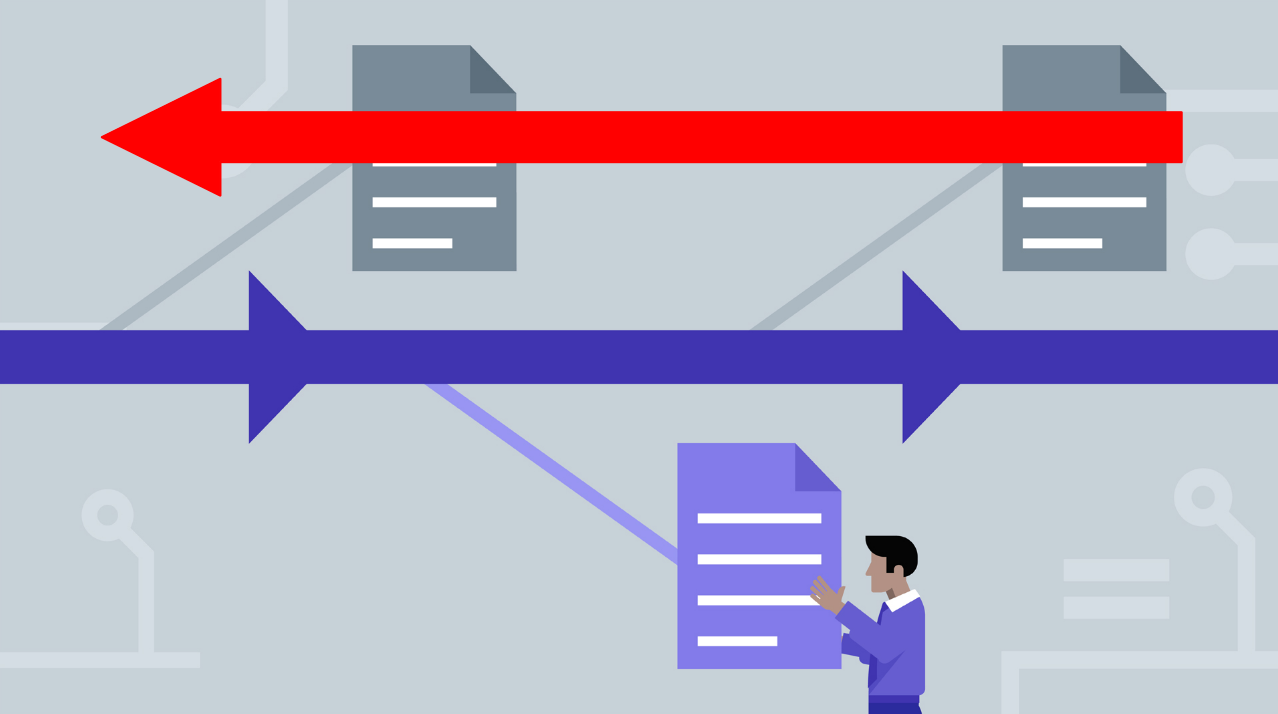
\includegraphics[scale=0.20]{img/storingVersion2.png}
\end{center}  

\end{frame}


\begin{frame}
\frametitle{Why version control is important?}
\textbf{Collaborations} (networking).

\begin{center}
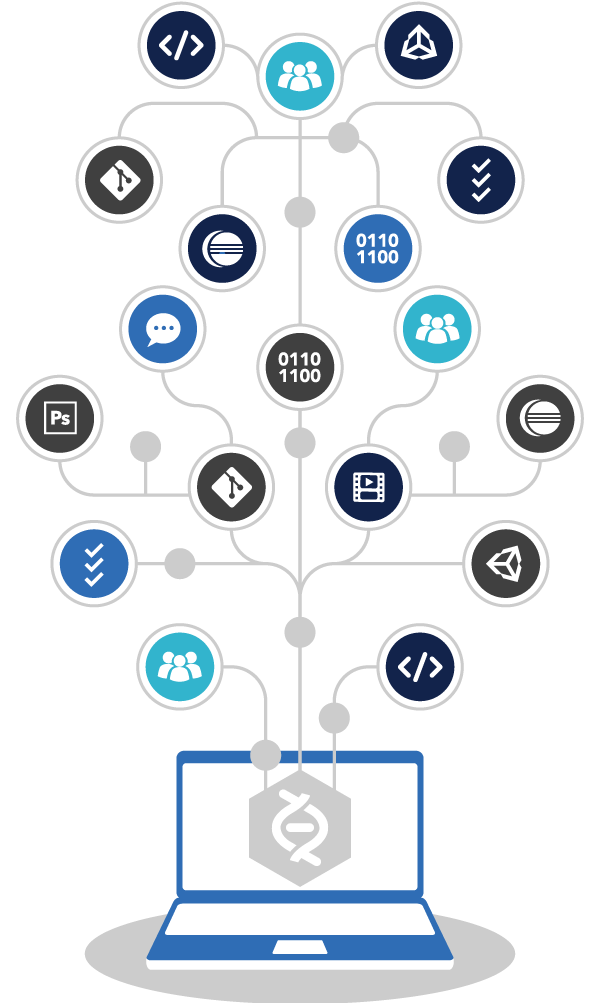
\includegraphics[scale=0.20]{img/networking.png}
\end{center}

\end{frame}


\begin{frame}
\frametitle{Why version control is important?}
Save \textbf{time}.

\begin{center}
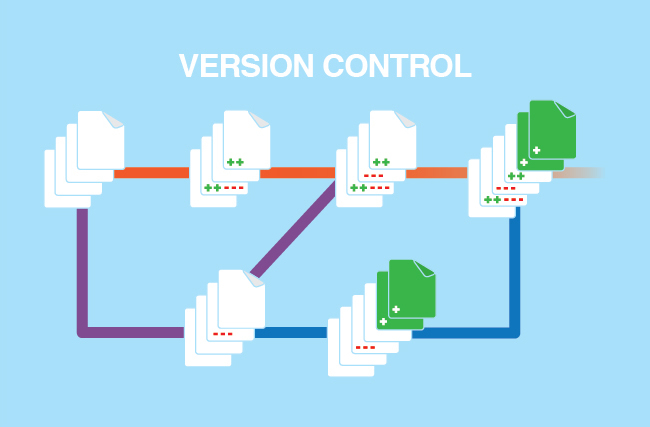
\includegraphics[scale=0.35]{img/version-control.png}
\end{center}

\end{frame}


\begin{frame}
\frametitle{Version control software}

\begin{center}
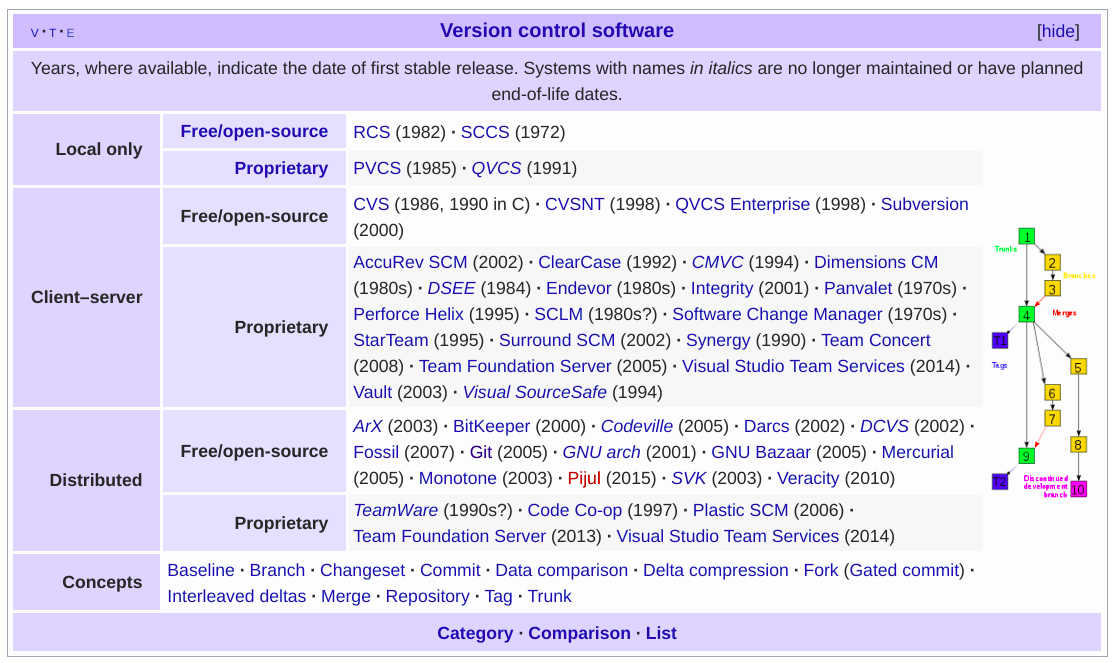
\includegraphics[scale=0.29]{img/controlVersion.png}
\end{center}

\end{frame}

\begin{frame}
    \frametitle{What is Git?}

    \textbf{Git} is a distributed version control system for tracking changes in source code during the development of software.

    \hfill \break

    \begin{center}
        
\includegraphics[scale=0.07]{img/git_logo.png}
    \end{center}
\end{frame}


\begin{frame}
    \frametitle{Why use Git?}
    \begin{itemize}
        \item \textbf{Popular and successful}
            \begin{itemize}
                \item[$-$]{Active development}
                \item[$-$]{Fast}
                    \hfill \break
            \end{itemize}

        \item \textbf{Distributed}
            \begin{itemize}
                \item[$-$]{Work online and offline}
                \item[$-$]{Collaborate with large groups}
                    \hfill \break
            \end{itemize}

        \item \textbf{Tracks any type of file}
            \begin{itemize}
                \item[$-$]{Works best with text}
                    \hfill \break
            \end{itemize}

        \item \textbf{Branching}
            \begin{itemize}
                \item[$-$]{Smarter merges}
            \end{itemize}
    \end{itemize}
\end{frame}


\begin{frame}
    \frametitle{What is GitHub Inc.?}

    \begin{center}
        \textbf{GitHub} is a web-based hosting service for version control using \textbf{Git}.
    \end{center}

    \begin{center}
        
\includegraphics[scale=0.2]{img/github_logos.png}
    \end{center}
\end{frame}


\begin{frame}
\frametitle{GitHub Inc.}
  \begin{itemize}
  \item Access to the control and collaboration features for every \textbf{project}.
  \end{itemize}

\begin{center}
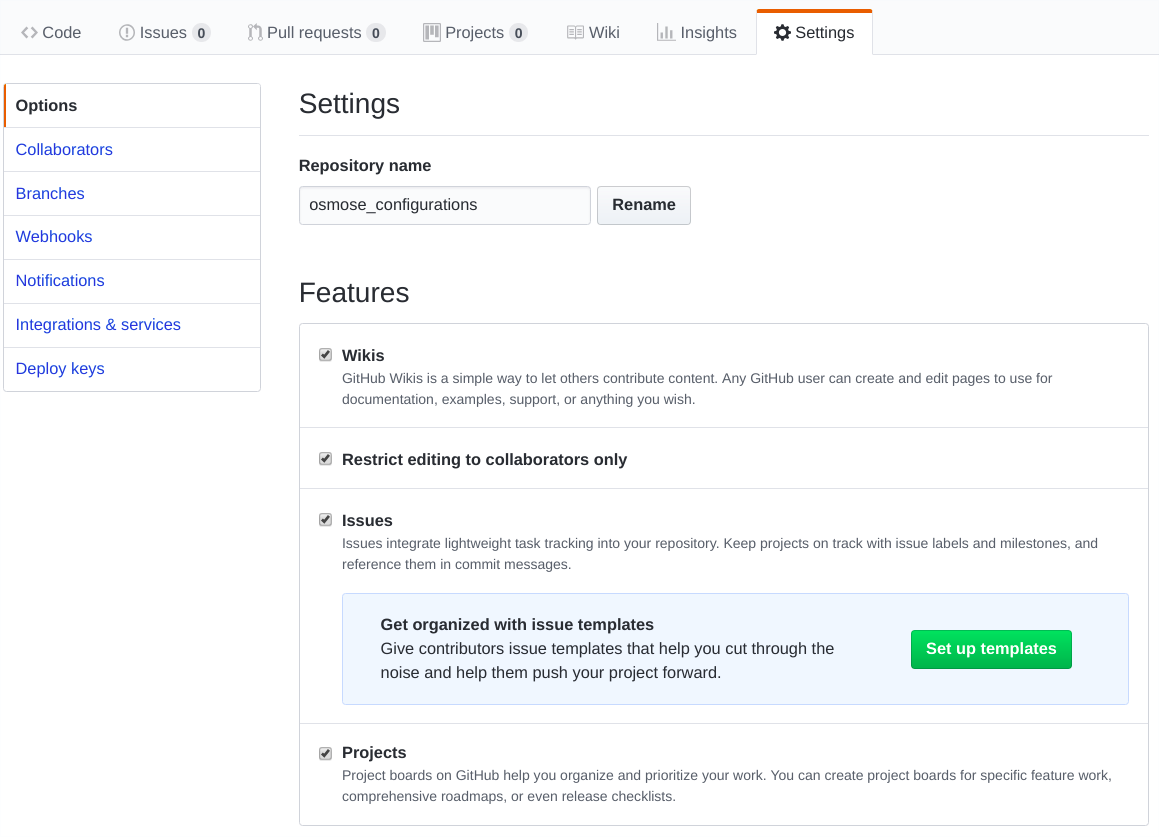
\includegraphics[scale=0.25]{img/githubRepo_settings.png}
\end{center}   

\end{frame}


\begin{frame}
\frametitle{GitHub Inc.}
  \begin{itemize}
  \item Work with public and private \textbf{repositories}. 
  \end{itemize}

\begin{center}
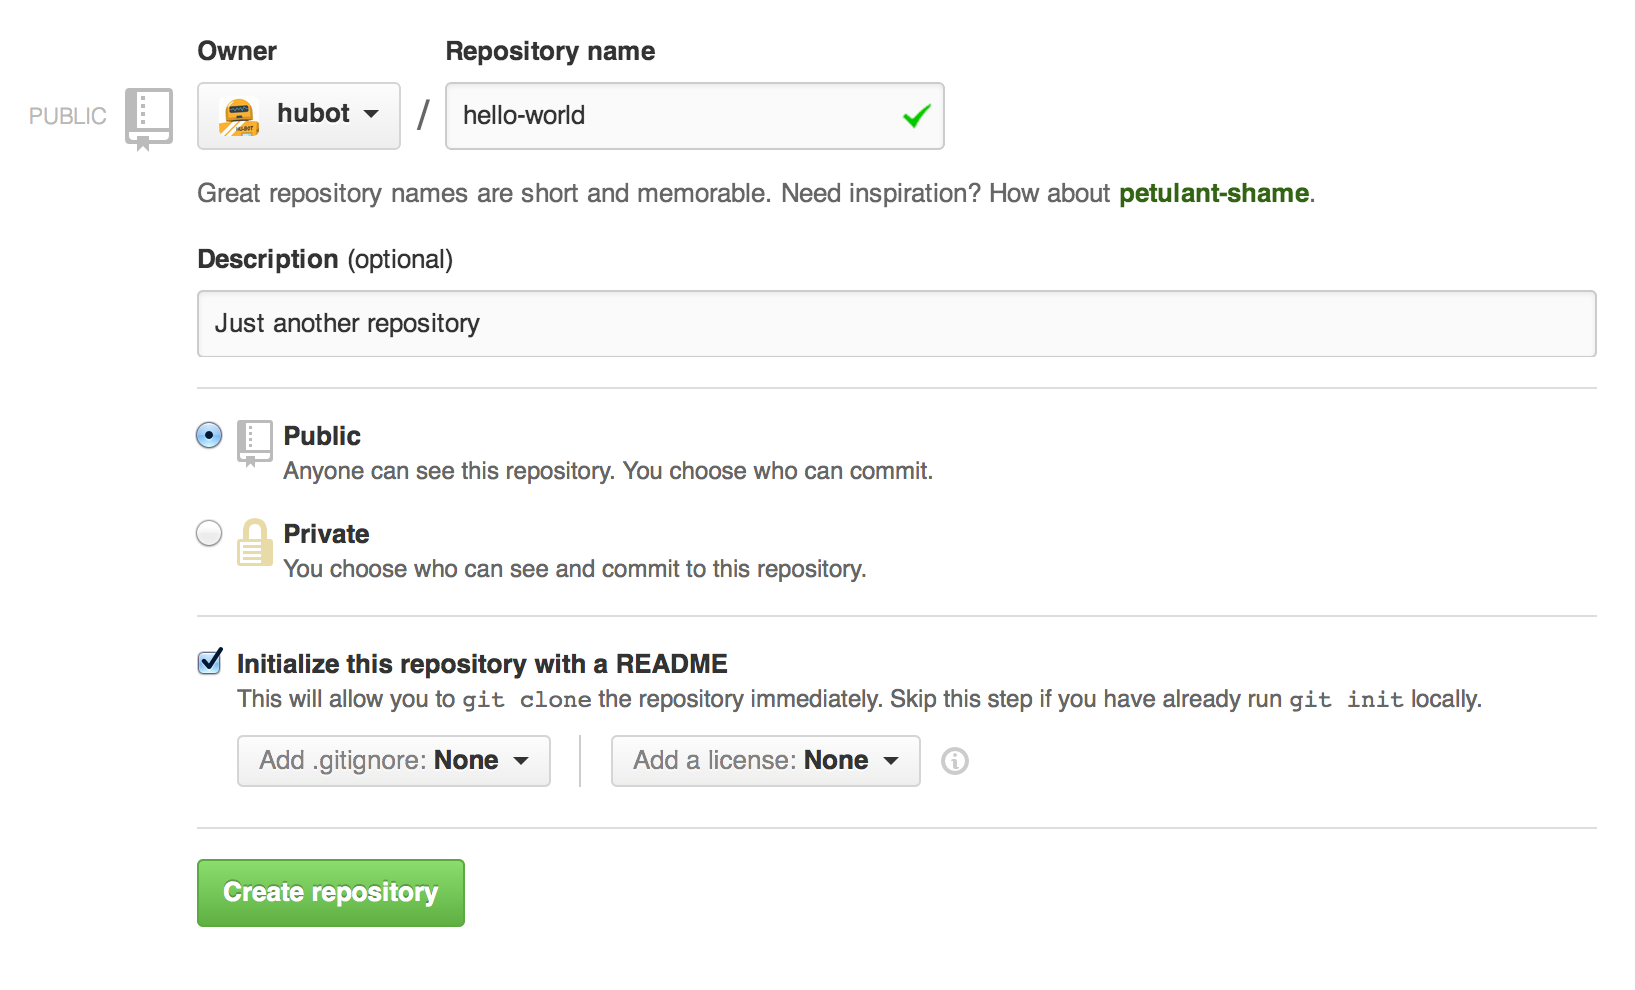
\includegraphics[scale=0.2]{img/githubRepo_features.png}
\end{center}  

\end{frame}


\begin{frame}
\frametitle{GitHub Inc.}
\begin{itemize}
  \item Develop a \textbf{networking}.
\end{itemize}

\begin{center}
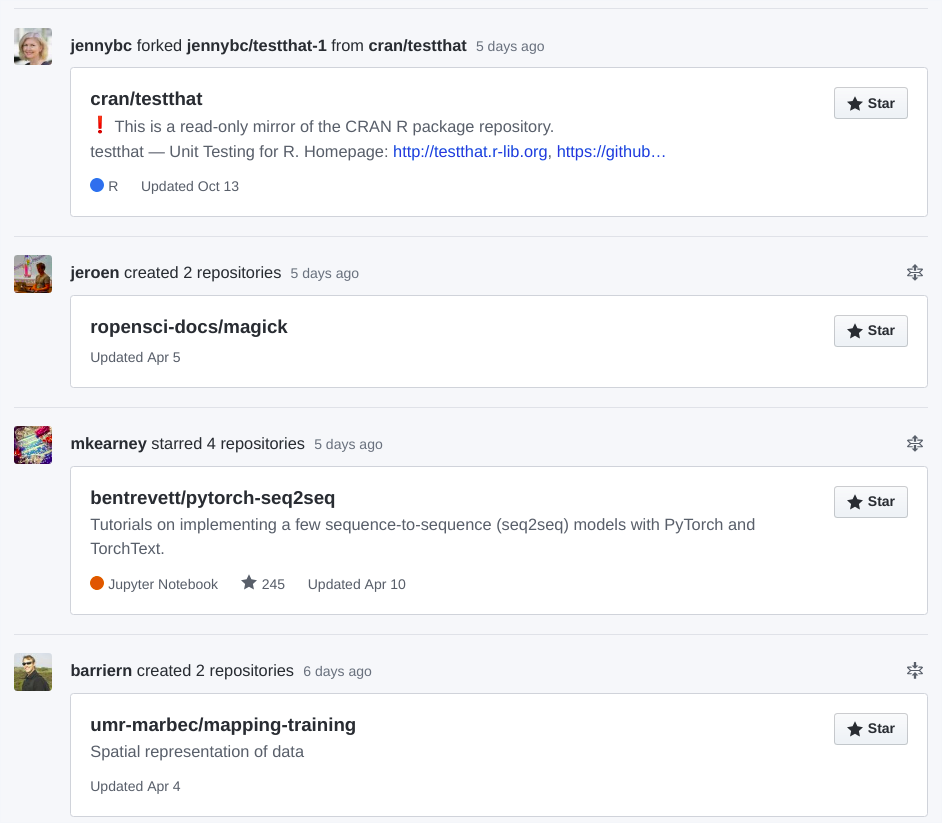
\includegraphics[scale=0.30]{img/githubRepo_networking.png}
\end{center}  

\end{frame}


\begin{frame}
    \frametitle{GitHub Inc.}
    \begin{itemize}
        \item \textbf{Plans} for enterprise, teams, pro and free accounts. \hfill \break
    \end{itemize}

\begin{center}

\includegraphics[scale=0.20]{img/github_plans.png}
\end{center}  


\end{frame}


\begin{frame}
\frametitle{GitHub Inc.}
\begin{itemize}
\item Is the \textbf{largest} host of source code in the world! \emph{(28 million users, 57 million repositories (28 million public) - June 2018)}.
\end{itemize}

\begin{center}

\includegraphics[scale=0.35]{img/microsoft-github-800x421.png}
\end{center}  

\end{frame}


\begin{frame}
\frametitle{Register a GitHub account}
  \begin{itemize}
    \item Create an account in \href{https://github.com/}{ GitHub} is free! \hfill \break
    \item Free private repositories
        \begin{itemize}
        \item[$-$] Students, faculty, and educational / research staff: \href{https://education.github.com/}{ GitHub Education}.
        \item[$-$] Official nonprofit organizations and charities: \href{https://github.com/nonprofit}{ GitHub for Good}.
       \end{itemize}
        
\end{itemize}
\end{frame}

\begin{frame}
\frametitle{Register a GitHub account}
\begin{itemize}
    \item Pay for private repositories
    \begin{itemize}
    \item[$-$] Individual cost is 7 dollars per month: \href{https://github.com/pricing}{ GitHub Pricing}.
    \end{itemize}

\end{itemize}

\begin{center}
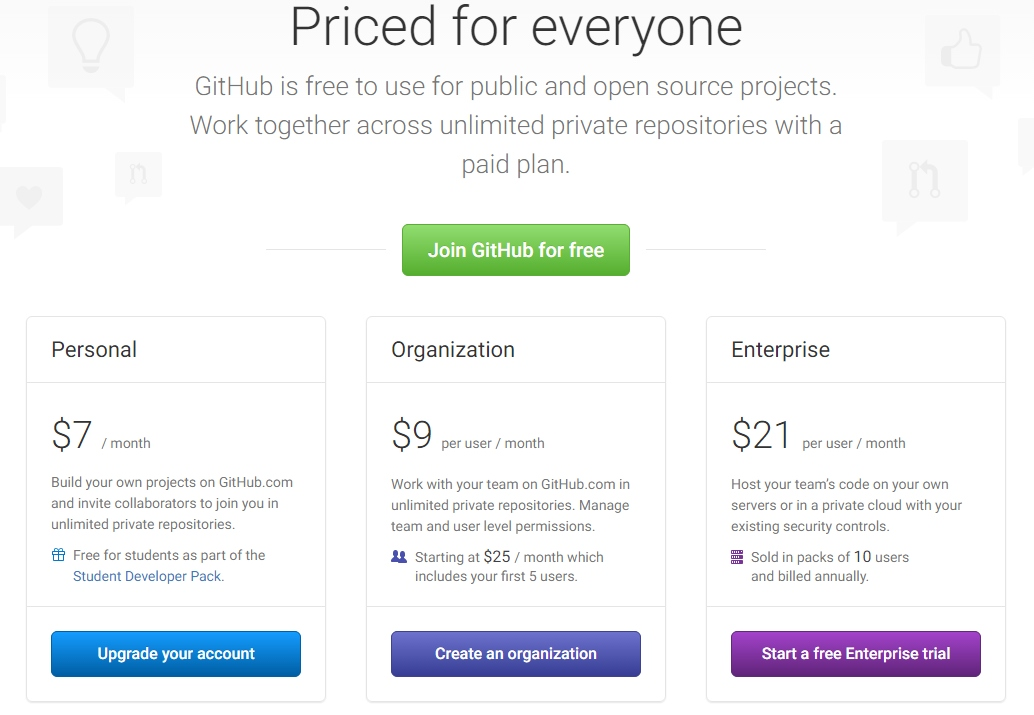
\includegraphics[scale=0.35]{img/github_pricing.jpg}
\end{center}  
\end{frame}

\begin{frame}
\frametitle{Marbec in GitHub}

    All the materials of Pole Modelisation's technical "workshop" are now stored in an institutionnal GitHub account: \url{https://github.com/umr-marbec}.

\begin{center}
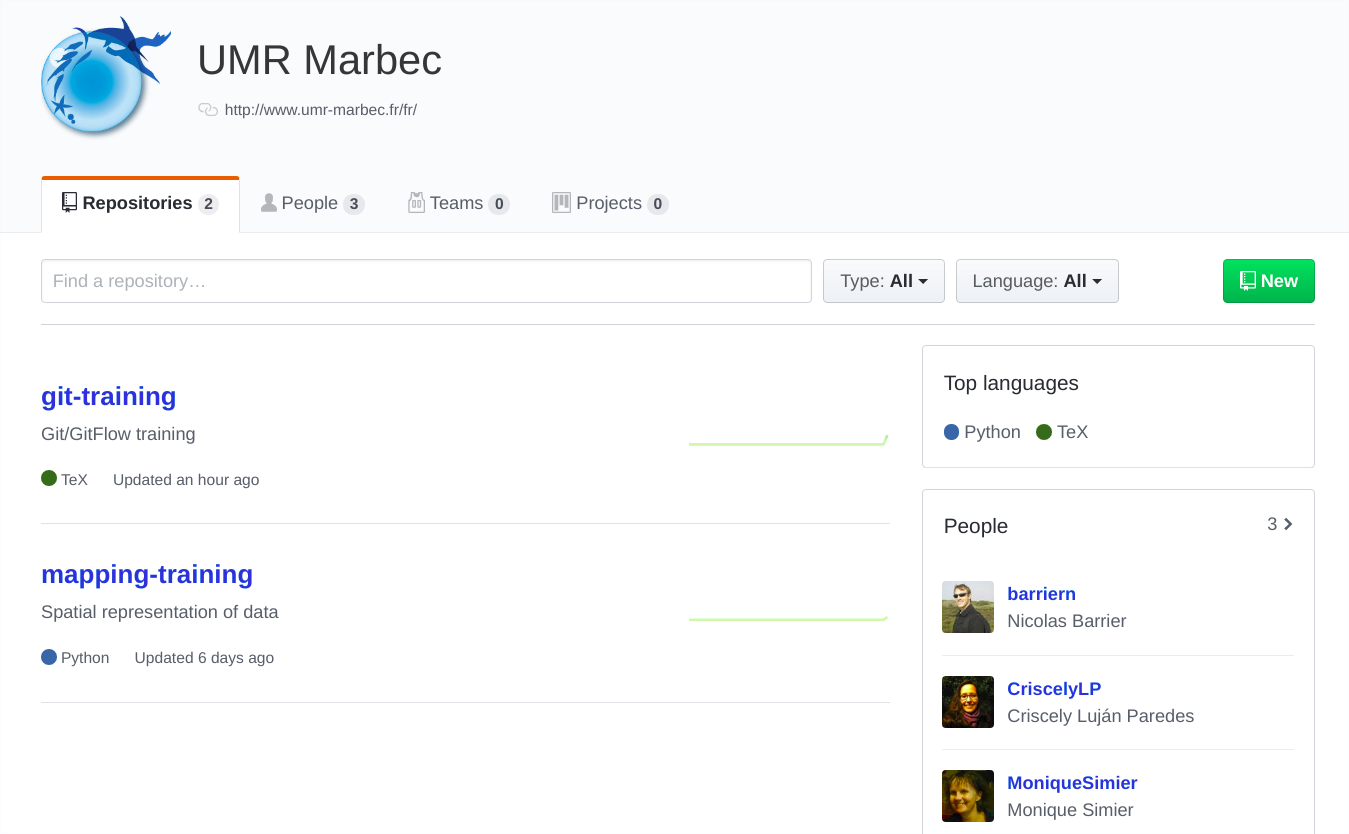
\includegraphics[scale=0.2]{img/github_marbec.png}
\end{center}  
\end{frame}

\begin{frame}
    \frametitle{Institutionnal repositories}

    GitHub is a private US company. There are also \emph{institutional} repositories on which Git can be used:

    \begin{itemize}
        \item{\href{https://sourcesup.renater.fr/}{Sourcesup}: this is a Renater platform (login possible from any French research institute or through CRU accounts)}
        \item{\href{https://forge.ifremer.fr/}{Forge Ifremer}: very close to SourceSup (Ifremer extranet account required)}
        \item{\href{gitlab.intranet.ird.fr}{IRD GitLab}: GitLab IRD platform (IRD account required).}
    \end{itemize}

    However, the projects hosted on these repositories may have less visibility...

\end{frame}


\begin{frame}
    \frametitle{Git clients}

    Git and Git client \textbf{are not} the same! Like R and RStudio is not the same thing!
    \hfill \break

    Git client:
    \begin{itemize}
        \item IDE (Integrated development environment)!
        \item Make the experience more pleasant providing a richer visual representation.
    \end{itemize}

    \hfill 

    Some example of Git clients:
    \begin{itemize}
        \item \href{https://www.sourcetreeapp.com/}{ SourceTreen} 
        \item \href{https://www.gitkraken.com/}{ GitKraken}
        \item \href{https://gitup.co/}{ GitUp} 
        \item \href{https://www.syntevo.com/smartgit/}{ SmartGit} 
        \item \href{https://git-cola.github.io/}{ git-cola} 
        \item \href{https://www.rstudio.com/}{ RStudio}
    \end{itemize}

    \vspace{3em}

\end{frame}

\begin{frame}[fragile]
    \frametitle{Git branches}
    One main advantage of Git is the use of \emph{branches}, which allow multiple developments of the same code at the same time.

    \begin{block}{Definition}
        A branch in Git is simply a lightweight movable pointer to one of thes commits.
    \end{block}
    
    \begin{center}
        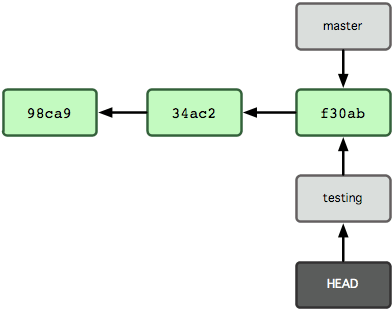
\includegraphics[height=2.5cm]{img/git-branch-ter.png}
        \hspace{3em}
        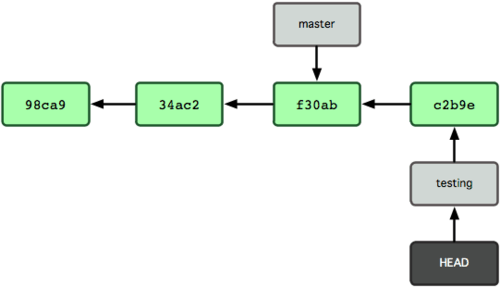
\includegraphics[height=2.5cm]{img/git-branch-bis.png}
    \end{center}

    In this example, the \verb+master+ branch points to the \verb+f30ab+ commit, while the \verb+testing+ branch points to the \verb+c2b9e+ one. \verb+HEAD+ points
    to the active branch (here, \verb+testing+).

    \vspace{1em}
    \tiny Source: \url{https://git-scm.com/book/en/v1/Git-Branching-What-a-Branch-Is}

\end{frame}

\begin{frame}[fragile]
    \frametitle{Merging branches}
    To merge a branch (for instance a feature branch) to another branch (for instance the main one), several options are offered.
    \begin{itemize}
        \item{\verb+merge+: Three-points branch (common ancestor + tips of the two branches)} 
        \item{\verb+rebase+: Compresses all the changes into a single “patch.” }
    \end{itemize}

    \begin{center}
        \begin{figure}
            \subfloat[Merge]{
                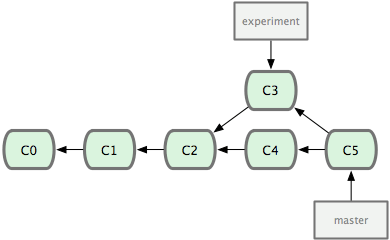
\includegraphics[scale=0.3]{img/git-merge-1.png}
                \label{git-merge}
            }
            \hspace{3em}
            \subfloat[Rebase]{
                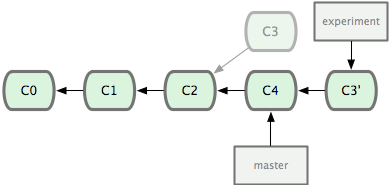
\includegraphics[scale=0.3]{img/git-merge-2.png}
                \label{git-rebase}
            }
            \caption{Merging versus rebasing}
        \end{figure}
    \end{center}

    \tiny Source: \url{https://git-scm.com/book/fr/v1/Les-branches-avec-Git-Rebaser}

\end{frame}

\begin{frame}
    \frametitle{Git workflows} % Table of contents slide, comment this block out to remove it
    There are several ways to use Git branches (we talk about \textbf{workflows}). 

    \begin{itemize}
        \item \emph{Centralized workflow}: one main branch, everyone commit in the same place.
        \item \emph{Feature Branch Workflow}: developments are made in dedicated branches (feature branches), which are regularly merged into the master one.
        \item \textbf{\textit{Gitflow Workflow}}: Strict branching model designed around the project release.
    \end{itemize}

    \tiny Source: \url{https://www.atlassian.com/git/tutorials/comparing-workflows}

\end{frame}

\begin{frame}[fragile]{GitFlow branches}

    GitFlow workflow contains two main branches:
    \begin{itemize}
        \item{\verb+master+: official release history. Branch which is shared to the world!}
        \item{\verb+develop+: integration branch for features}
    \end{itemize}

    It also contains additional temporal branches:
    \begin{itemize}
        \item{\verb+feature+: feature branches (one for each new feature to add to the code)}
        \item{\verb+release+: branch created when enough features have been added (new version of the code) to develop}
        \item{\verb+hotfix+: branch for maintenance and bug correction of the production release}
    \end{itemize}

\end{frame}

\begin{frame}{In summary...}

    \begin{center}
        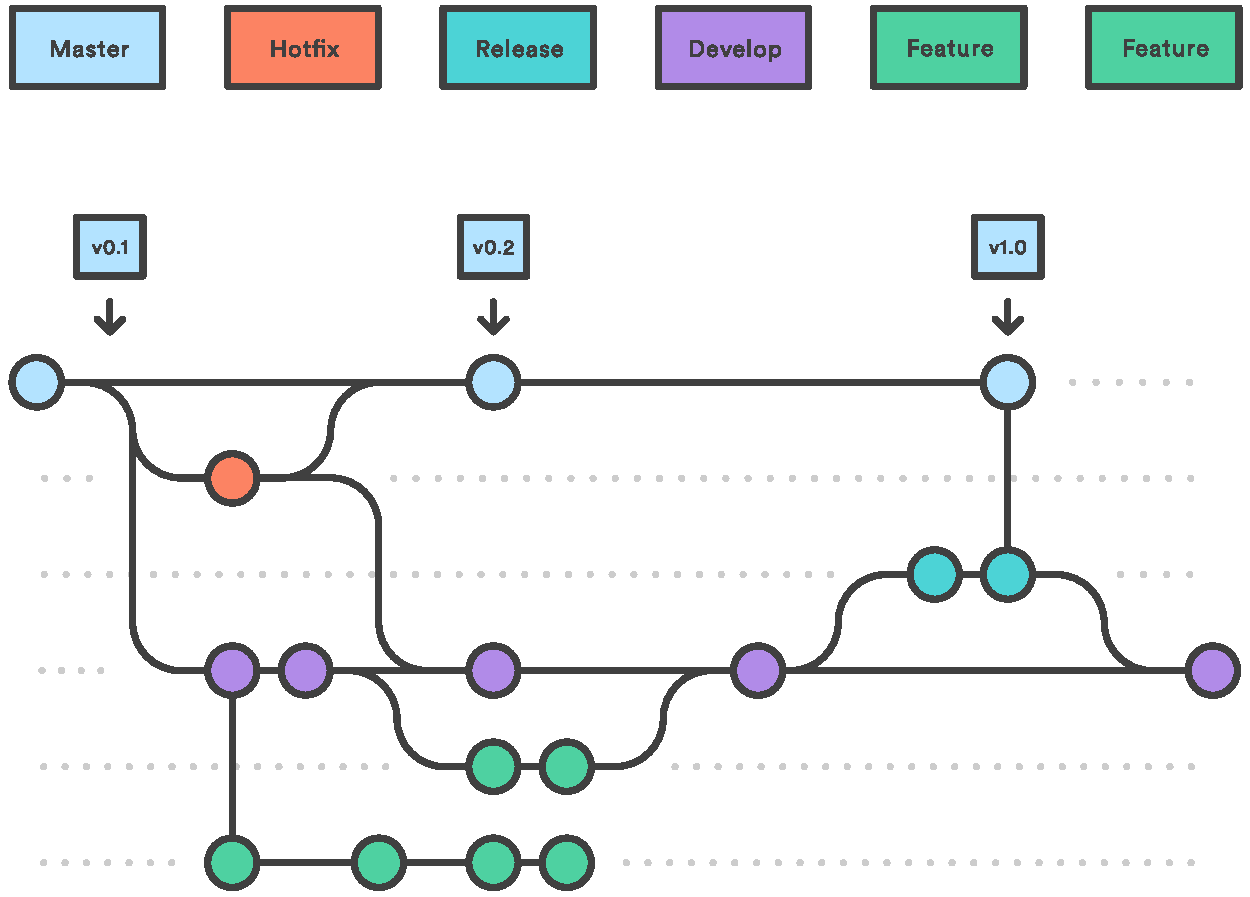
\includegraphics[scale=0.5]{img/05-_2_.pdf}    
    \end{center}
    
    \tiny Source: \url{https://www.atlassian.com/git/tutorials/comparing-workflows}

\end{frame}    


\begin{frame}
    \frametitle{Thanks for your attention} % Table of contents slide, comment this block out to remove it

            \begin{center}
                \textbf{Now, let's crack on it!}\\
                \vspace{2em}

                
\includegraphics[scale=0.15]{img/funny.jpg}\\
                \vspace{1em}
                \tiny Source: \url{https://www.pinterest.fr/pin/447263806724736402/}
            \end{center}
\end{frame}



\end{document}
